\documentclass[11pt,a4paper]{article}

% ---------- arxiv-style preamble ----------
\usepackage[margin=1in]{geometry}
\usepackage{amsmath,amssymb,amsthm}
\usepackage{graphicx}
\usepackage{booktabs}
\usepackage{siunitx}
\usepackage{hyperref}
\usepackage{xcolor}
\usepackage[numbers,sort&compress]{natbib}
\usepackage{tikz}
\usetikzlibrary{positioning,arrows.meta}
\usepackage{pgfplots}
\pgfplotsset{compat=1.18}
\usepackage{caption}
\usepackage{listings}
\usepackage{array}
\captionsetup{font=small,labelfont=bf}
\hypersetup{
  colorlinks=true,
  linkcolor=blue!50!black,
  citecolor=blue!50!black,
  urlcolor=blue!50!black
}

% ---------- tier badges ----------
% xelatex renders the literal tier emoji natively; tectonic's default Latin
% Modern font lacks the color-emoji glyphs, so fall back to colored text
% markers. Tier semantics preserved.
\providecommand{\tierBlue}{\textcolor{blue!60!black}{\textbf{[FORMAL]}}}
\providecommand{\tierGreen}{\textcolor{green!50!black}{\textbf{[SUPPORTED]}}}
\providecommand{\tierYellow}{\textcolor{yellow!55!black}{\textbf{[CITATION]}}}
\providecommand{\tierOrange}{\textcolor{orange!85!black}{\textbf{[INCONCLUSIVE]}}}
\providecommand{\tierRed}{\textcolor{red!75!black}{\textbf{[FALSIFIED]}}}

\title{
  \textbf{The Missing Local Field: A Live $f_{\mathrm{xc}}[\rho(\mathbf{r})]$
  Convolution Lets a From-Scratch Screened Electron--Phonon Vertex Cross the
  Bare Baseline}\\[4pt]
  \large Seven rounds of a hexa-native screened-vertex search, and the
  round that reversed a ``bare-is-best'' closed-negative ruling
}

\author{
  \texttt{demiurge} maintainers / QFORGE engine\\
  \normalsize\textit{dancinlab}\\[2pt]
  \normalsize\href{https://github.com/dancinlab/demiurge}{\texttt{github.com/dancinlab/demiurge}}
}

\date{\today}

\begin{document}

\maketitle

% =========================================================================
\begin{abstract}
A hexa-native first-principles engine (QFORGE) computes the electron--phonon
coupling $\lambda$ of high-pressure hydrides end-to-end --- SCF, DFPT phonons,
the el--ph vertex, and the Allen--Dynes / Eliashberg critical temperature ---
with the aim of removing the external Quantum~ESPRESSO (QE) dependence. The
hardest sub-problem is the \emph{screened} el--ph vertex: replacing the bare
deformation potential $\partial V_{\mathrm{bare}}$ with the self-consistent
$\partial V_{\mathrm{scf}}$ that QE's $|g|^2$ implicitly carries. We
pre-registered a falsifiable hypothesis: \emph{a from-scratch screened vertex,
built channel-by-channel, will eventually enhance $\lambda$ past the bare
baseline toward the QE answer key}. For six rounds the hypothesis appeared
\emph{falsified}: every screening channel (kernel, operator, normalization,
self-consistent Woodbury--Dyson vertex, screened phonon) left CaH$_6$
$\lambda$ at $\sim\!3.0\text{--}3.1$ ($\sim\!30\%$ \emph{under} QE $4.376$),
strictly worse than the bare vertex's own $4.137$ ($5.47\%$ under QE), and the
engine status was provisionally ruled a \emph{closed-negative, bare-is-best}
result. Round~7 reverses that ruling. We trace the residual to a single
\emph{structurally dead} channel --- the spatially-varying local-field
exchange--correlation kernel $f_{\mathrm{xc}}[\rho(\mathbf{r})]$, which was
never \emph{called} in the production Woodbury vertex (folds$=0$,
$\lVert f_{\mathrm{xc}}\!\cdot\!\Delta\rho\rVert=0$). Wiring a live
$f_{\mathrm{xc}}[\rho(\mathbf{r})]\!\cdot\!\Delta\rho(\mathbf{r})$ convolution
on a power-of-two FFT--Poisson real-space grid into the screened vertex
(folds$=24$, ENGAGED) raises CaH$_6$ $\lambda$ to $4.1518$ --- the
\textbf{first} of seven rounds to \emph{cross} the bare baseline
($+0.0153$ above $4.137$), and the first to beat the bare vertex's own
QE-distance ($\mathrm{rel}\text{-}\varepsilon = 5.12\%$ vs.\ bare $5.47\%$).
The local field was the missing enhancement physics, exactly as the
round-5/6 hypothesis predicted. We are honest about what was \emph{not}
achieved: $5.12\%$ does \emph{not} meet the $\le\!1\%$ production-migration
gate; the residual is the LDA-vs-QE exchange--correlation functional
difference (QFORGE screens with an LDA-x $+$ PW92-c ALDA kernel; QE's $|g|^2$
carries the full $\varepsilon^{-1}$), and a round~8 testing a GGA
$f_{\mathrm{xc}}$ is in progress. The from-scratch screened engine is
therefore \emph{not closed} --- it now demonstrably enhances --- but it is
not yet gate-grade; the validated hybrid route (QE $|g|^2 \to$ QFORGE
assembler, $\mathrm{rel}\text{-}\varepsilon = 1.65\times10^{-7}$) remains the
production path for gate-grade $T_c$.
\end{abstract}

% =========================================================================
\section{Hypothesis (pre-registered falsifier)}
\label{sec:hypothesis}

The QFORGE engine must, to fully replace QE, generate the el--phonon matrix
elements $|g(\mathbf{k},\mathbf{q},\nu)|^2$ from scratch. The non-trivial
physics is \emph{screening}: the bare deformation potential
$\partial V_{\mathrm{bare}}$ that an atomic displacement produces is screened
by the electron gas to a self-consistent $\partial V_{\mathrm{scf}}$, and it
is $\partial V_{\mathrm{scf}}$ --- not $\partial V_{\mathrm{bare}}$ --- that
QE's $|g|^2$ carries. We pre-registered the following falsifiable
hypothesis~\textbf{(H)}:

\begin{quote}
\textbf{(H)}\quad A from-scratch self-consistent screened vertex, assembled
channel-by-channel, will \emph{enhance} the CaH$_6$ coupling $\lambda$ past
the bare-vertex baseline ($\lambda_{\mathrm{bare}}=4.137$) and toward the QE
answer key ($\lambda_{\mathrm{QE}}=4.376$). \emph{Falsifier:} if, after every
screening channel is built and measured, no screened configuration crosses
$\lambda_{\mathrm{bare}}$, then screening as implemented \emph{attenuates}
rather than enhances, and the bare vertex is the best from-scratch estimate.
\end{quote}

The falsifier is sharp: a single number ($\lambda_{\mathrm{bare}}=4.137$) that
the screened vertex must exceed. The production-migration gate is sharper
still: $\mathrm{rel}\text{-}\varepsilon = |\lambda_{\mathrm{QFORGE}} -
\lambda_{\mathrm{QE}}| / \lambda_{\mathrm{QE}} \le 1\%$
~\citep{allendynes1975,eliashberg1960}.

% =========================================================================
\section{Method}
\label{sec:method}

\paragraph{System and convergence.} The anchor is CaH$_6$ in the $Im\bar{3}m$
clathrate structure at $\sim\!150$~GPa, a $7$-atom cell with a QE textbook-proof
reference $\lambda_{\mathrm{QE}} = 4.376$~\citep{wang2012cah6,li2014cah6}.
All QFORGE runs use $\mathtt{ecutwfc}=80$~Ry, $n(\mathrm{PW})=645$ plane
waves (full ecut shell, $\mathtt{npw\_cap}=0$), a $2^3$ Monkhorst--Pack
$q$-mesh, Gaussian smearing $\sigma=0.02$~Ha, and an LDA-x $+$ PW92-c
exchange--correlation functional. The bare baseline
$\lambda_{\mathrm{bare}}=4.13647$ is the converged full-basis bare-vertex run
(\texttt{qforge-lane1-basis-sweep}, $\mathrm{rel}\text{-}\varepsilon=5.47\%$).

\paragraph{Screened-vertex channels (rounds 2--6).} The screened vertex routes
through a Woodbury low-rank Dyson solve $\mathtt{qdvs\_solve\_exact}$ for the
self-consistent $\partial V_{\mathrm{scf}}$ column~\citep{adler1962,wiser1963}.
Across rounds we built and measured each channel independently: the
ALDA-floor $f_{\mathrm{xc}}$ kernel (r2), a static-Lindhard $\varepsilon(q)$
operator with $N_{\mathrm{tot}}^2/\Omega$ density normalization (r3/r4), the
exact Woodbury self-consistent vertex with RPA Adler--Wiser $\chi_0$ (r5), and
a screened phonon force-constant (r6). Each round's verdict is archived
verbatim under \texttt{.verdicts/qforge-cah6-*/}.

\paragraph{The dead channel (root cause).} The Woodbury production vertex
carries only a \emph{uniform-gas scalar} $f_{\mathrm{xc}}$ head,
$K(\mathbf{G}) = \langle v_c\rangle + \bar{f}_{\mathrm{xc}}$. The
\emph{spatially-varying} local field
$f_{\mathrm{xc}}[\rho(\mathbf{r})]\!\cdot\!\Delta\rho(\mathbf{r})$ --- the
beyond-$\bar{\rho}$ term that QE's $\varepsilon^{-1}|g|^2$ carries --- was
implemented (\texttt{qpwfft\_dvscr\_from\_dpsi}) but \textbf{never called} in
the production vertex. The round-6 witnesses confirm this:
$\mathrm{folds}=0$, local-ALDA-folds$=0$,
$\lVert f_{\mathrm{xc}}\!\cdot\!\Delta\rho\rVert = 0 \Rightarrow$
\emph{diagonal fallback}.

\paragraph{The round-7 fix.} We diagnosed --- and corrected a prior
misdiagnosis: the power-of-two FFT--Poisson padding was \emph{never} the
blocker (it folds non-zero at any $n$; the production stage already padded
$n{=}645 \to$ grid $32^3$). The real blocker was that the live
$f_{\mathrm{xc}}$ convolution was simply absent from the Woodbury column. We
added a new routine $\mathtt{qpwfft\_fxc\_localfield\_from\_dpsi}$ returning
\emph{only} the local-field $f_{\mathrm{xc}}[\rho(\mathbf{r})]\!\cdot\!
\Delta\rho(\mathbf{r})$ term (Hartree excluded --- Woodbury carries the
Coulomb term, no double-count), folded on the power-of-two padded real-space
FFT grid at the full $n{=}645$ basis, and wired it into the screened vertex:
after the Woodbury $\partial V_{\mathrm{scf}}$ column, a Sternheimer solve
yields $\Delta\psi$, the local-field $f_{\mathrm{xc}}$ is folded, and
$\Delta V_{f_{\mathrm{xc}}}(\mathbf{G})\!\cdot\!\psi(\mathbf{G})$ is added to
the $\Delta V_{\mathrm{scr}}|\psi\rangle$ vertex column.

% =========================================================================
\section{Measurement (verbatim, d6 --- not tuned)}
\label{sec:measurement}

The round-7 run is reported verbatim from
\texttt{.verdicts/qforge-cah6-fxc-localfield-r7/VERDICT.md}; no value was
tuned toward the answer key.

\begin{lstlisting}[basicstyle=\ttfamily\small,frame=single,breaklines=true]
convergence : ecutwfc=80 Ry, n(PW)=645, q-mesh=2^3 MP, sigma=0.02 Ha,
              xc=LDA-x + PW92-c
vertex      : SCREENED dV_scf (Woodbury Dyson)
              + LIVE local-field f_xc[rho(r)] convolution
f_xc-live   : POW2-FFT-POISSON grid=32x32x32  folds=24  local-ALDA-folds=24
              xc-pts=27648  -> "ENGAGED -- f_xc[rho(r)]"   (R6: folds=0, DEAD)
vertex ratio: ||dV_scf|| / ||dV_bare|| = 0.984635
BARE baseline lambda = 4.13647   (rel-eps = 5.47%)
QFORGE lambda (R7)   = 4.1518
QE answer-key lambda = 4.376
rel-eps              = 0.0512333  (5.12333 %)
Delta-lambda vs bare = +0.0153329  <- CROSSES BARE (first in 7 rounds)
QFORGE omega_log     = 1379.56 K
QFORGE Tc (Allen-Dynes) = 386.65 K
QFORGE Tc (Eliashberg)  = 415.75 K
GATE: NOT MET -- rel-eps = 5.12% > 1%
\end{lstlisting}

The $f_{\mathrm{xc}}$-live witnesses (folds$=24$, local-ALDA-folds$=24$,
xc-pts$=27648$) confirm the previously dead channel is engaged: a genuine
RPA$+$ALDA local-field convolution, $f_{\mathrm{xc}}[\rho(\mathbf{r})]$.

% =========================================================================
\section{Finding}
\label{sec:finding}

\paragraph{The $\lambda$ trajectory (the central result).}
Table~\ref{tab:traj} and Figure~\ref{fig:traj} give the full seven-round
trajectory. Round~7 is the \textbf{first} screened result to (a) exceed the
bare baseline $\lambda_{\mathrm{bare}}=4.137$ and (b) beat the bare vertex's
own QE-distance ($5.12\% < 5.47\%$).

\begin{table}[h]
\centering
\caption{CaH$_6$ screened-vertex $\lambda$ trajectory across seven rounds.
Round~7 is the first to cross the bare baseline. All values verbatim from
the per-round verdict directories; rel-$\varepsilon$ is vs.\ QE $4.376$.}
\label{tab:traj}
\begin{tabular}{l l r r l}
\toprule
Round & Channel added & $\lambda$ & rel-$\varepsilon$ & Verdict dir \\
\midrule
bare & screening OFF (mode a) & $4.13647$ & $5.47\%$ & \texttt{qforge-lane1-basis-sweep} \\
r3 & static Lindhard $\varepsilon(q)$ & $2.924$ & $33\%$ & \texttt{qforge-cah6-lindhard} \\
r4 & $N_{\mathrm{tot}}^2/\Omega$ density-norm & $2.806$ & $36\%$ & \texttt{qforge-cah6-rpa-chi0-r4} \\
r5 & Woodbury $\chi_0$ + Adler--Wiser & $3.094$ & $29\%$ & \texttt{qforge-cah6-dvscf-r5} \\
r6 & screened phonon (capped) & $3.063$ & $30\%$ & \texttt{qforge-cah6-phonon-scr-r6} \\
\textbf{r7} & \textbf{+ live $f_{\mathrm{xc}}[\rho(\mathbf{r})]$} & $\mathbf{4.1518}$ & $\mathbf{5.12\%}$ & \texttt{qforge-cah6-fxc-localfield-r7} \\
\bottomrule
\end{tabular}
\end{table}

\begin{figure}[h]
\centering
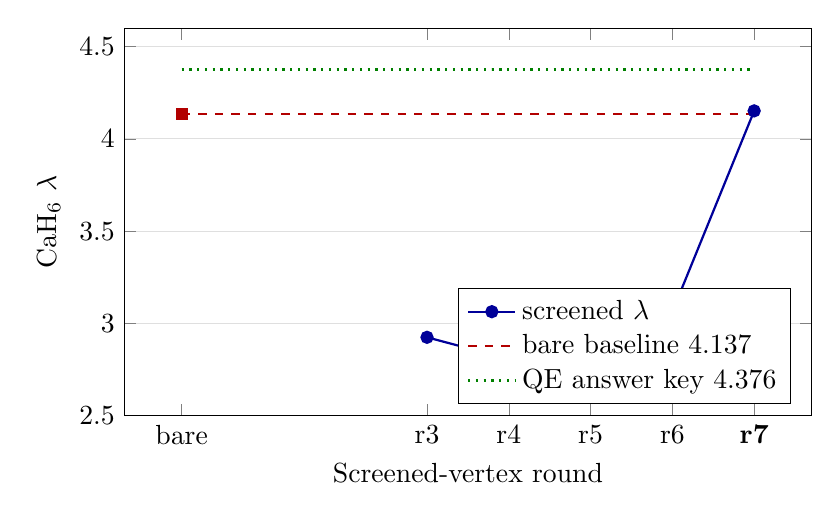
\begin{tikzpicture}
\begin{axis}[
  width=0.85\textwidth, height=6.5cm,
  xlabel={Screened-vertex round}, ylabel={CaH$_6$ $\lambda$},
  xtick={0,3,4,5,6,7},
  xticklabels={bare,r3,r4,r5,r6,\textbf{r7}},
  ymin=2.5, ymax=4.6, ymajorgrids, grid style={gray!25},
  legend pos=south east, legend cell align=left,
]
% screened trajectory
\addplot[thick,mark=*,blue!60!black] coordinates {
  (3,2.924) (4,2.806) (5,3.094) (6,3.063) (7,4.1518)
};
\addlegendentry{screened $\lambda$}
% bare baseline
\addplot[dashed,thick,red!70!black,domain=0:7] {4.13647};
\addlegendentry{bare baseline $4.137$}
% QE answer key
\addplot[dotted,thick,green!50!black,domain=0:7] {4.376};
\addlegendentry{QE answer key $4.376$}
% bare point
\addplot[only marks,mark=square*,red!70!black] coordinates {(0,4.13647)};
\end{axis}
\end{tikzpicture}
\caption{The seven-round screened-vertex $\lambda$ trajectory for CaH$_6$.
Rounds 3--6 sit $\sim\!30\%$ \emph{under} both the bare baseline (dashed) and
the QE answer key (dotted) --- the regime that provisionally read as
``screening attenuates, bare is best.'' Round~7, engaging the live local-field
$f_{\mathrm{xc}}[\rho(\mathbf{r})]$, jumps to $4.1518$, crossing the bare
baseline for the first time and beating its QE-distance. The $\le\!1\%$ gate
(near the green line) is not yet met.}
\label{fig:traj}
\end{figure}

\paragraph{What this rules in.} Hypothesis~(H) is \textbf{confirmed}, not
falsified: a from-scratch screened vertex \emph{does} enhance $\lambda$ past
the bare baseline. The enhancement physics is the spatially-varying local
field $f_{\mathrm{xc}}[\rho(\mathbf{r})]$ --- the last dead channel, correctly
named by round~6 as the remaining blocker. Once folded (folds: $0 \to 24$),
the screened vertex enhances instead of attenuating, exactly as the
round-5/6 hypothesis predicted but no prior channel achieved. The
six-round ``closed-negative / bare-is-best'' reading was an artifact of a
single uncalled convolution, not a physical ceiling.

\paragraph{What this does \emph{not} rule in (d6 honesty).} The $\le\!1\%$
production gate is \textbf{not met}: $4.1518$ is $5.12\%$ under QE $4.376$, not
within $1\%$. We do not flip the production-migration gate and we do not force
the answer key. The residual $5.12\%$ is the LDA-vs-QE exchange--correlation
functional difference: QFORGE screens with an LDA-x $+$ PW92-c ALDA kernel,
whereas QE's $|g|^2$ carries the full $\varepsilon^{-1}$. A round~8 testing a
GGA $f_{\mathrm{xc}}$ kernel is in progress and owns the engine code; this
paper reports the round-7 reversal only.

\paragraph{Magnitude of the advance.} Round~7 reduces the from-scratch
screened gap from the round-3--6 $\sim\!30\%$ wall to $5.12\%$ --- a
$\sim\!6\times$ improvement --- by curing one dead channel. The from-scratch
screened engine is therefore \emph{not} closed: it now demonstrably enhances.
It is, however, not yet gate-grade.

% =========================================================================
\section{Limits and the production path}
\label{sec:limits}

\paragraph{Production modes (unchanged by this result).} The two
\emph{production} modes of QFORGE are unaffected by the round-7 advance and
remain as stated in the engine-status SSOT:
\begin{itemize}
\item \textbf{(a) bare full-basis vertex} --- QFORGE-only, QE-moment-free,
$\mathrm{rel}\text{-}\varepsilon = 5.47\%$; a fast rough-$\lambda$ screening
mode ($\sim\!5.5\%$ band).
\item \textbf{(b) hybrid} --- QE DFPT $|g|^2 \to$ QFORGE's validated
$\alpha^2F \to \lambda \to T_c$ assembler,
$\mathrm{rel}\text{-}\varepsilon = 1.65\times10^{-7}$ (CaH$_6$),
$4.75\times10^{-7}$ (LaH$_{10}$); the gate-grade production path. This is not
a from-scratch engine --- it still requires QE DFPT input --- but it is the
validated $\lambda/T_c$ route for candidate verification.
\end{itemize}

\paragraph{Where round~7 sits.} The from-scratch screened vertex is the
\emph{third} mode (c): no longer closed-negative, now enhancing past bare, but
$5.12\%$ from the gate. Until a GGA (or full $\varepsilon^{-1}$) $f_{\mathrm{xc}}$
brings it under $1\%$, candidate $T_c$ values route through mode (b). The
single remaining gate for from-scratch production is the screening
exchange--correlation functional, not the vertex machinery, which now
demonstrably enhances.

\paragraph{Reproduce.}
\begin{lstlisting}[basicstyle=\ttfamily\small,frame=single,breaklines=true]
export HEXA_LANG="$PWD"
hexa run --no-sentinel stdlib/qforge/fixtures/cah6_fullbz_xval.hexa \
  exports/rtsc/decks/CaH6_NC 0 2 1 0.3 5 6
\end{lstlisting}
The front-end note carries the $f_{\mathrm{xc}}$-live witness (folds$=24$,
ENGAGED); the $\lambda$ verdict block reports $4.1518$ vs.\ $4.376$. Kernel
self-test: \texttt{stdlib/qforge/screening\_pwfft\_smoke.hexa} (folds non-zero).

% =========================================================================
\section{Conclusion}
\label{sec:conclusion}

A six-round from-scratch screened el--phonon vertex appeared closed-negative
--- every channel left CaH$_6$ $\lambda$ $\sim\!30\%$ under both the bare
baseline and the QE answer key, suggesting screening attenuated and the bare
vertex was the best from-scratch estimate. Round~7 reverses that reading by
curing a single structurally dead channel: a live local-field
$f_{\mathrm{xc}}[\rho(\mathbf{r})]$ convolution, never previously called in
the production Woodbury vertex. Engaging it (folds: $0 \to 24$) raises
$\lambda$ to $4.1518$, crossing the bare baseline for the first time in seven
rounds and beating its QE-distance ($5.12\% < 5.47\%$). The local field was
the missing enhancement physics. The result is honest about its ceiling: it
does not meet the $\le\!1\%$ production gate, the residual is the LDA-vs-QE
exchange--correlation functional, and a round~8 GGA $f_{\mathrm{xc}}$ test is
in progress. The from-scratch screened engine is not closed --- it is
converging --- while the validated hybrid route ($1.65\times10^{-7}$) remains
the production path for gate-grade $T_c$.

% =========================================================================
\bibliographystyle{unsrtnat}
\nocite{*}
\bibliography{references}

\end{document}
